% Brilliant documentation:
% http://mirror.ox.ac.uk/sites/ctan.org/macros/latex/contrib/beamer/doc/beameruserguide.pdf

\usepackage{beamerthemesplit}
\usepackage{tikz}
\usetikzlibrary{arrows.meta,shapes,backgrounds,positioning,shapes.multipart}
\usepackage{textpos} 
\usepackage{hyperref}
\usepackage{graphicx}
\usepackage{calc}
%\usepackage[usenames,dvipsnames,svgnames,table]{xcolor} PACKAGE CLASH!
%\usepackage{color}
\newlength{\popupimagewidth}

\setlength{\popupimagewidth}{\textwidth*3/5}

\addtobeamertemplate{frametitle}{}{
  % From http://tex.stackexchange.com/a/180628
  \begin{textblock*}{100mm}(\textwidth,-1cm)
    
\includegraphics[height=1cm,width=1cm]{ise-logo.jpg}
  \end{textblock*}
}

\title{Linked Open Data in Action}
\author{Matt Wallis}
\date{\today}

% From http://tex.stackexchange.com/a/183966:
\tikzset{
    invisible/.style={opacity=0,text opacity=0},
    visible on/.style={alt=#1{}{invisible}},
    alt/.code args={<#1>#2#3}{%
      \alt<#1>{\pgfkeysalso{#2}}{\pgfkeysalso{#3}} % \pgfkeysalso doesn't change the path
    },
}

\begin{document}

\frame{
  \begin{center}
    Download handout now

    http://

    Twitter: \href{https://twitter.com/SolidarityEcon}{@SolidarityEcon}
  \end{center}
}
\frame{\titlepage}

\frame{\tableofcontents}

\section{Institute for Solidarity Economics}
\frame
{
  \frametitle{Institute for Solidarity Economics}
  \begin{center}
    
\includegraphics[height=2cm,width=2cm]{ise-logo.jpg}
  \end{center}
  \begin{itemize}
    \item<1-> \url{http://solidarityeconomics.org}
    \item<1-> The Solidarity Economy is a grassroots movement that is building a fair and ecological alternative to Capitalism.
    \item<1-> Our aim is to support this movement through education, research, and finding opportunities for collaboration.
  \end{itemize}
}
\subsection{Why data?}
\frame
{
  \frametitle{Why data?}
  \begin{itemize}
    \item Help people find what's out there -- e.g. Maps
    \item Behind every map is data
    \item Behind every app is data
    \item 
  \end{itemize}
}
Here's something between frames that appears only in the article.
\frame
{
  \frametitle{Guiding Principles}
  \begin{itemize}
    \item Data ownership is power - be careful!
    \item Prefer distributed to centralized data
    \item Prefer appropriate ownership of data
    \item Trust is vital - make sources of data visible
    \item Don't Repeat Yourself! (DRY)
    \item Use existing best practice
    \item Re-use existing software
  \end{itemize}
}
Our work is available on GitHub: \url{https://github.com/p6data-coop/ise-linked-open-data}
\section{What we did}
\frame
{
  \frametitle{Research}
  \begin{itemize}
    \item Linked Open Data looked like best practice
    \item But scary! {\em we didn't really understand it}
    \item Experimentation
      \begin{itemize}
	\item Co-ops UK dataset (open, CSV)
	\item Use existing ESSGLOBAL vocabulary
	\item Learn about Linked Open Data
	\item Generate experimental LOD dataset of over 13,000 UK Co-ops
	\item Put them on a map
      \end{itemize}
    \item 
  \end{itemize}
}
\frame
{
  \frametitle{Development}
  \begin{itemize}
    \item Generate experimental LOD dataset of over 13,000 UK Co-ops
    \item Put them on a map
    \item Document and educate
  \end{itemize}
}
\subsection{Linked Open Data}
%\frame[fragile,t]
\frame[t]
{
  \frametitle{Passing links as data}
  \centering
  %\begin{center}
  %\begin{tikzpicture}[scale=.8, show background rectangle, node distance=1cm]
  %\begin{tikzpicture}[remember picture, show background rectangle, node distance=1cm]
  \begin{tikzpicture}[remember picture, node distance=1cm]
    \tikzstyle{every text node part} = [align=center]
    \tikzstyle{obj node} = [ellipse, fill=blue!20]
    \tikzstyle{obj path} = [->, draw=blue!20]
    \tikzstyle{label node} = [draw, text=black]
    \tikzstyle{data node} = [rectangle, fill=green!20]
    \tikzstyle{extdata node} = [rectangle, draw, fill=green!20]
    \tikzstyle{app node} = [rectangle, fill=red!20]
    %\tikzstyle{label node} = [near start, sloped, auto]
    \tikzstyle{label node} = [midway, auto]
    \tikzstyle{label text} = [align=left]
    \node[obj node] (iseobj) {\underline{Links to other datasets} e.g. \\ {\visible<2->{http://os.gov/postcode/OX10AB}} \\ {\visible<3->{http://ch.gov/company/12345678}}};
    \node[label text, visible on=<1->] (datalabel) [left = of iseobj] {Example \\ data:};
    \node[extdata node, visible on=<2->] (osdata) [below = of iseobj ] {OS data};
    \node[data node] (isedata) [left = of osdata] {Our data};
    \node[extdata node, visible on=<3->] (chdata) [right = of osdata] {CH data};
    \node[label text, visible on=<1->] (datasetlabel) at (isedata-|datalabel) {Datasets:};

    %\node[obj node] (iseobj) [above = of chdata] {\underline{Data links to other datasets} e.g. \\ {\visible<2->{http://os.gov/postcode/OX10AB}} \\ {\visible<3->{http://ch.gov/company/12345678}}};
    \node[app node, visible on=<4->] (mapapp) [below left = of osdata] {Map};
    \node[app node, visible on=<5->] (nearestapp) [below right = of osdata] {Nearest};
    %\node[label text, visible on=<4->] (appslabel) [below = of datasetlabel, left = of mapapp] {Apps:};
    \node[label text, visible on=<4->] (appslabel) at (mapapp-|datasetlabel) {Apps:};
    %\path[obj path] (isedata) edge (iseobj.south);
    \draw[->, visible on=<1->] (isedata) -- (iseobj) node[label node]{contains};
    \draw[->, visible on=<2->] (iseobj) -- (osdata) node[midway, left]{link};
    \draw[->, visible on=<3->] (iseobj) -- (chdata) node[midway, right]{link};
    \draw[<->, visible on=<4>] (mapapp) -- (isedata) node[midway, right]{query};
    \draw[<->, visible on=<4>] (mapapp) -- (osdata) node[midway, right]{query};
    \draw[->, visible on=<5->] (mapapp) -- (nearestapp) node[midway, below]{http://ch.gov/...};
    \draw[<->, visible on=<5->] (nearestapp) -- (osdata) node[midway, left]{query};
    \draw[<->, visible on=<5->] (nearestapp) -- (chdata) node[midway, right]{query};
  \end{tikzpicture}
  %\end{center}
  %\begin{itemize}
    %\item
  %\end{itemize}
}

\frame
{
  \frametitle{ESSGLOBAL}
  \begin{itemize}
    \item
  \end{itemize}
}
\section{Applications}
\subsection{Example map application}
\frame
{
  \frametitle{map-app}
  \begin{itemize}
    \item Web application: \url{http://data.solidarityeconomics.org/map-app/}
    \item Data is loaded by querying our Linked Open Database (aka a Triple Store)
    \item Clean separation of application and data
  \end{itemize}
}
\frame
{
  \frametitle{Links in practice}
  \begin{center}
    %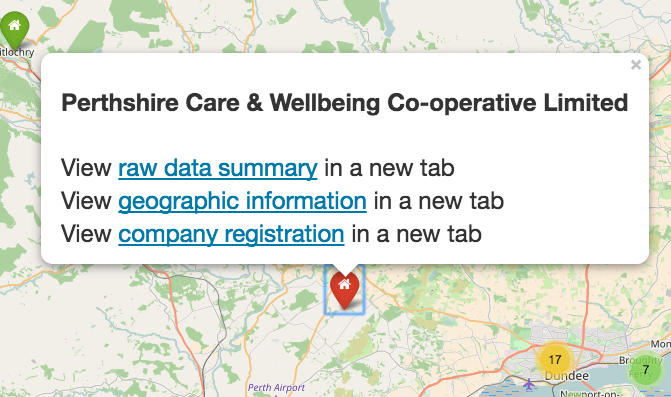
\includegraphics{map-app-popup-screenshot.png}
    \makebox[\textwidth]{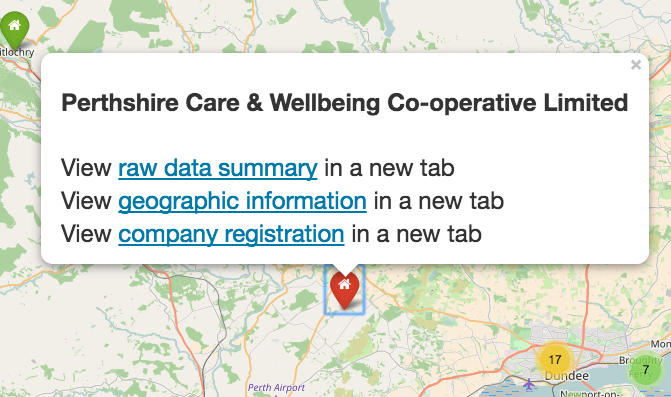
\includegraphics[width=\popupimagewidth]{map-app-popup-screenshot.png}}
    %\makebox[\textwidth]{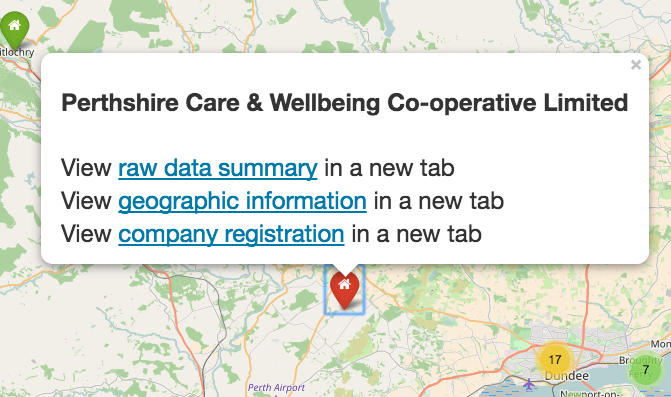
\includegraphics[width=\paperwidth]{map-app-popup-screenshot.png}}
    %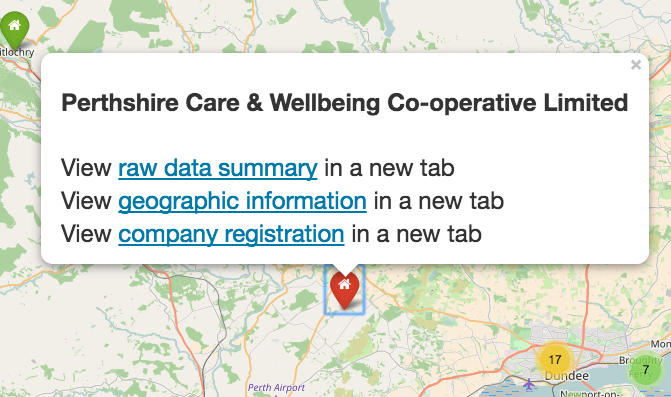
\includegraphics[height=2cm,width=2cm]{map-app-popup-screenshot.png}
  \end{center}
  \begin{itemize}
    \item
  \end{itemize}
}
\subsection{Power of LOD}
\frame
{
  \frametitle{Query across datsets}
  \begin{itemize}
    \item SPARQL demo
  \end{itemize}
}

\section{Conclusions}
\frame
{
  \frametitle{Lessons from re-use}
  \begin{itemize}
    \item Makes the original developers very happy
    \item Great co-operation from original developers
    \item Learn from others
    \item Answers questions you'd not know to ask \texttt{!important;}
    \item Leave things in better shape
  \end{itemize}
}
\frame
{
  \frametitle{LOD Everywhere?}
  \begin{center}
    %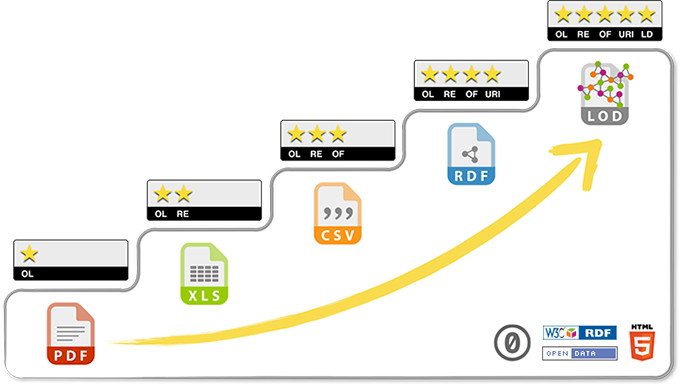
\includegraphics{5-star-steps.png}
    \makebox[\textwidth]{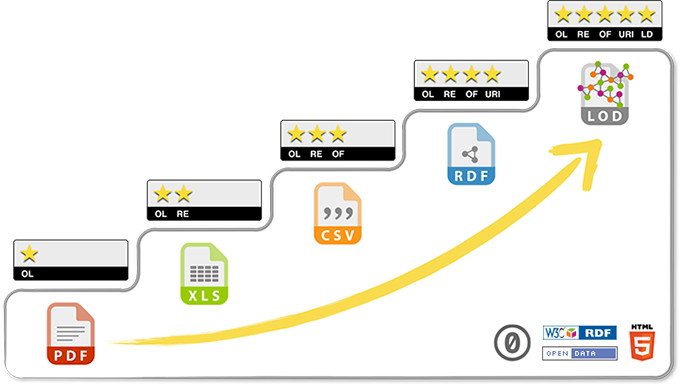
\includegraphics[width=\popupimagewidth]{5-star-steps.png}}
    %\makebox[\textwidth]{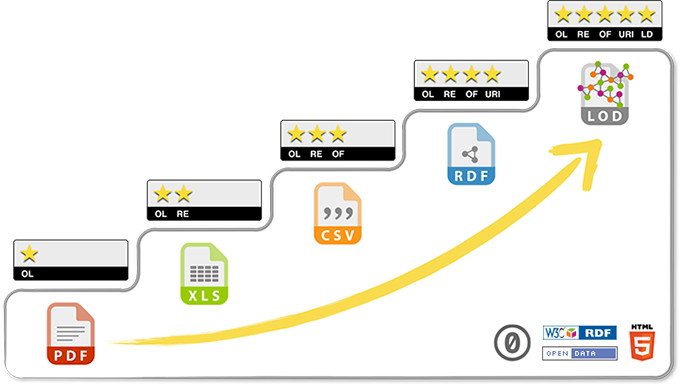
\includegraphics[width=\paperwidth]{5-star-steps.png}}
    %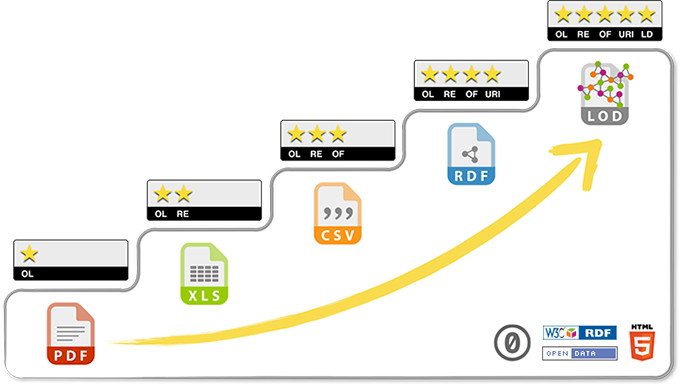
\includegraphics[height=2cm,width=2cm]{5-star-steps.png}
  \end{center}
  \begin{itemize}
    \item \url{http://5stardata.info}
  \end{itemize}
}
\frame
{
  \frametitle{The LOD approach}
  \begin{itemize}
    \item Avoid reinvention of wheels you didn't know existed
    \item Excellent for ``National Grid'' of data
    \item Easliy integrate with other data standards
    \item LOD everywhere? No!

  \end{itemize}
}
\frame
{
  \frametitle{What's next?}
  \begin{itemize}
    \item We can help
    \item How to find out more?
  \end{itemize}
}


\end{document}
